\section{Networking and privacy}\label{sec:net}

\subsection{Routes}

The person chooses one of three routes in first-boot setup: the Nym mixnet, which is the default; the Anyone onion network; or Direct. One library, \code{nonos\_route\_link}, holds the rule for every program that opens its own connections. Direct is used only when Direct is chosen, Anyone goes through \code{net.anon}, and anything else, an unreadable setting included, goes through Nym. A chosen network that is not running means no route, and nothing falls back.\srcs{userland/nonos_route_link/src/pick.rs:130-139}{docs/using/privacy-network.md} The wallet's chain reads and broadcasts never go Direct: under a Direct default they go over Nym, or over Anyone when Nym is not running, and with neither up there is no route.\src{userland/nonos_route_link/src/pick.rs:86-100} Downloads for installs use Anyone whatever the default, because Nym's exits end long streams part way and Anyone's circuits carry gigabytes.\src{userland/nonos_route_link/src/pick.rs:46-60} Host names travel unresolved to the exit, so no clear DNS query leaves the machine. Network drivers draw a new locally administered MAC address at each bring-up.\srcs{docs/using/privacy-network.md}{userland/nonos_mac/src/local.rs:46-55}

\begin{figure}[t]
\centering
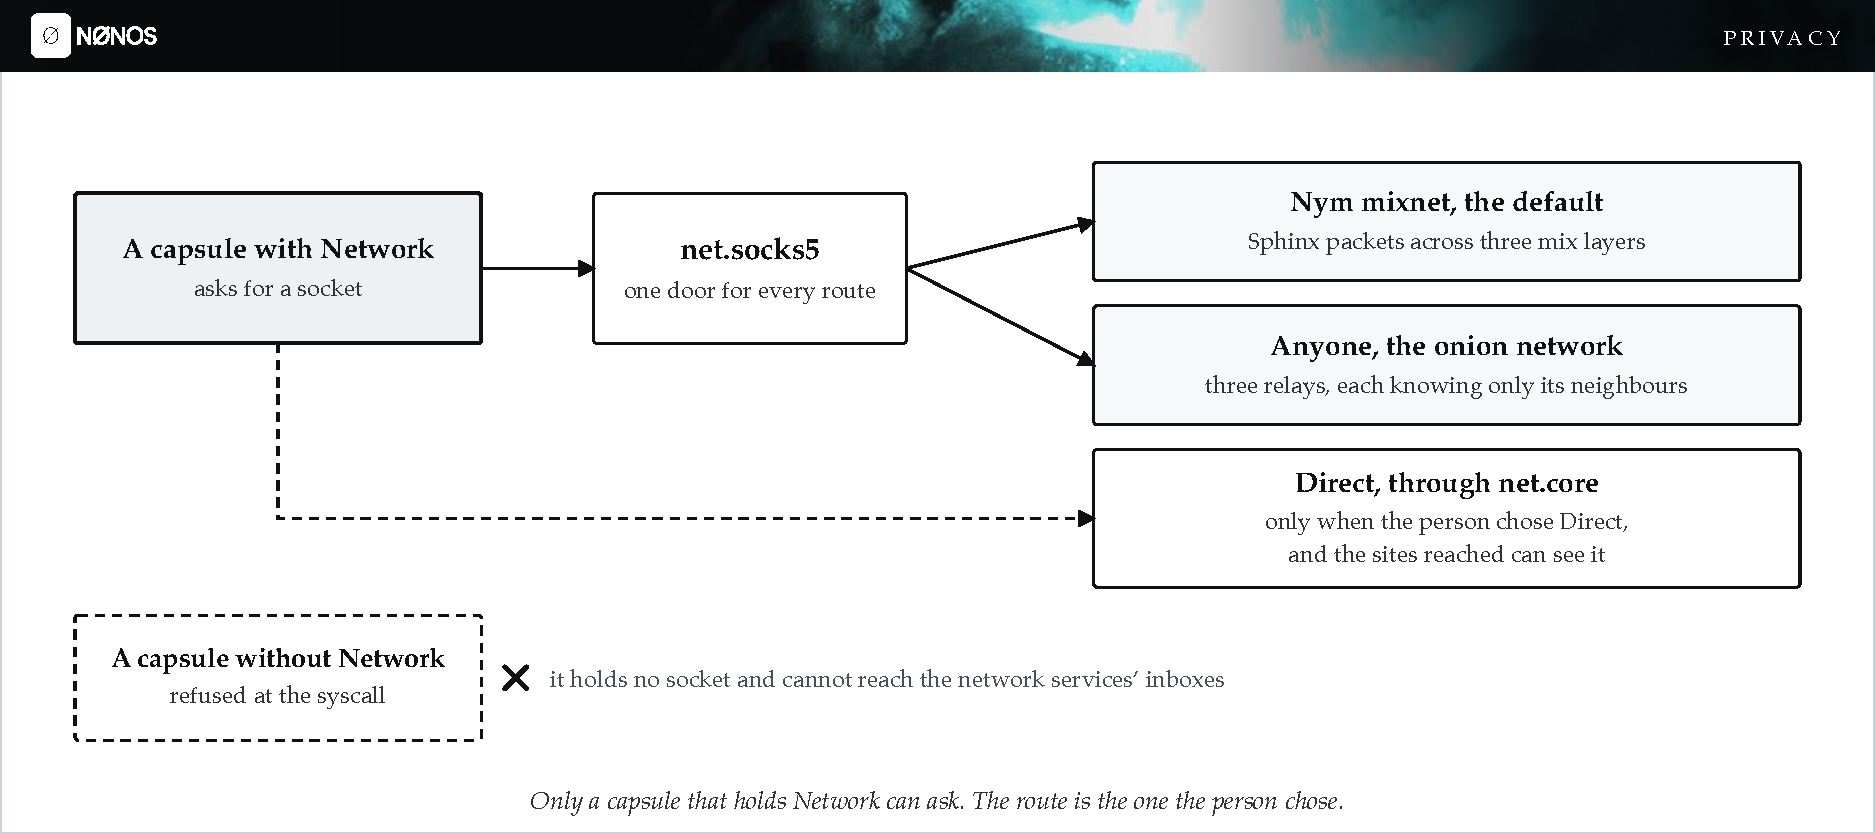
\includegraphics[width=0.84\textwidth]{figures/diagram-network-routes.pdf}
\caption{How a program's traffic leaves the machine. A capsule that holds \code{Network} asks \code{nonos\_route\_link} for a route; Nym streams go through \code{net.socks5} and \code{net.nym}, Anyone streams through \code{net.anon}, and Direct through \code{net.sockets}. A capsule without \code{Network} cannot reach the network services' inboxes. A Linux program in a box with \code{NET\_ANON} takes the same library's route and is never given Direct. Sources: \code{docs/using/privacy-network.md}, \code{src/services/registry/policy.rs}.}
\label{fig:routes}
\end{figure}

\begin{figure}[t]
\centering
\begin{minipage}[t]{0.40\textwidth}
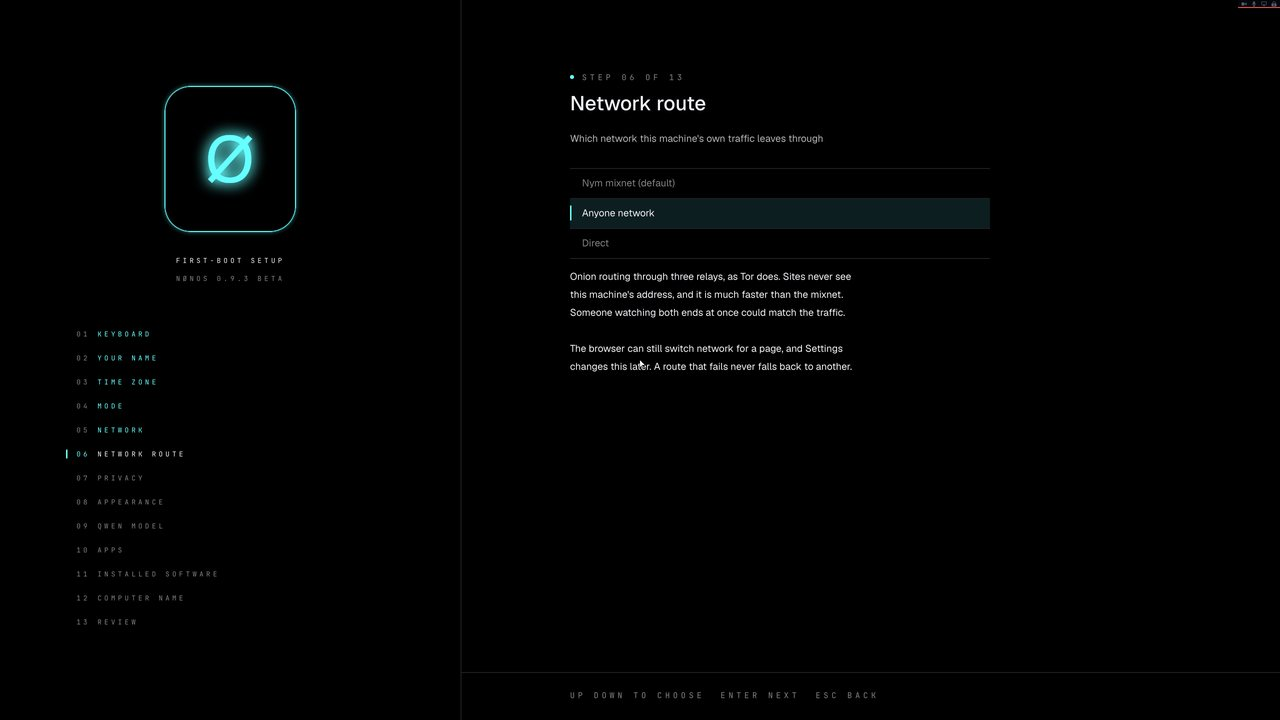
\includegraphics[width=\textwidth]{figures/setup-route.jpg}
\end{minipage}\hfill
\begin{minipage}[t]{0.40\textwidth}
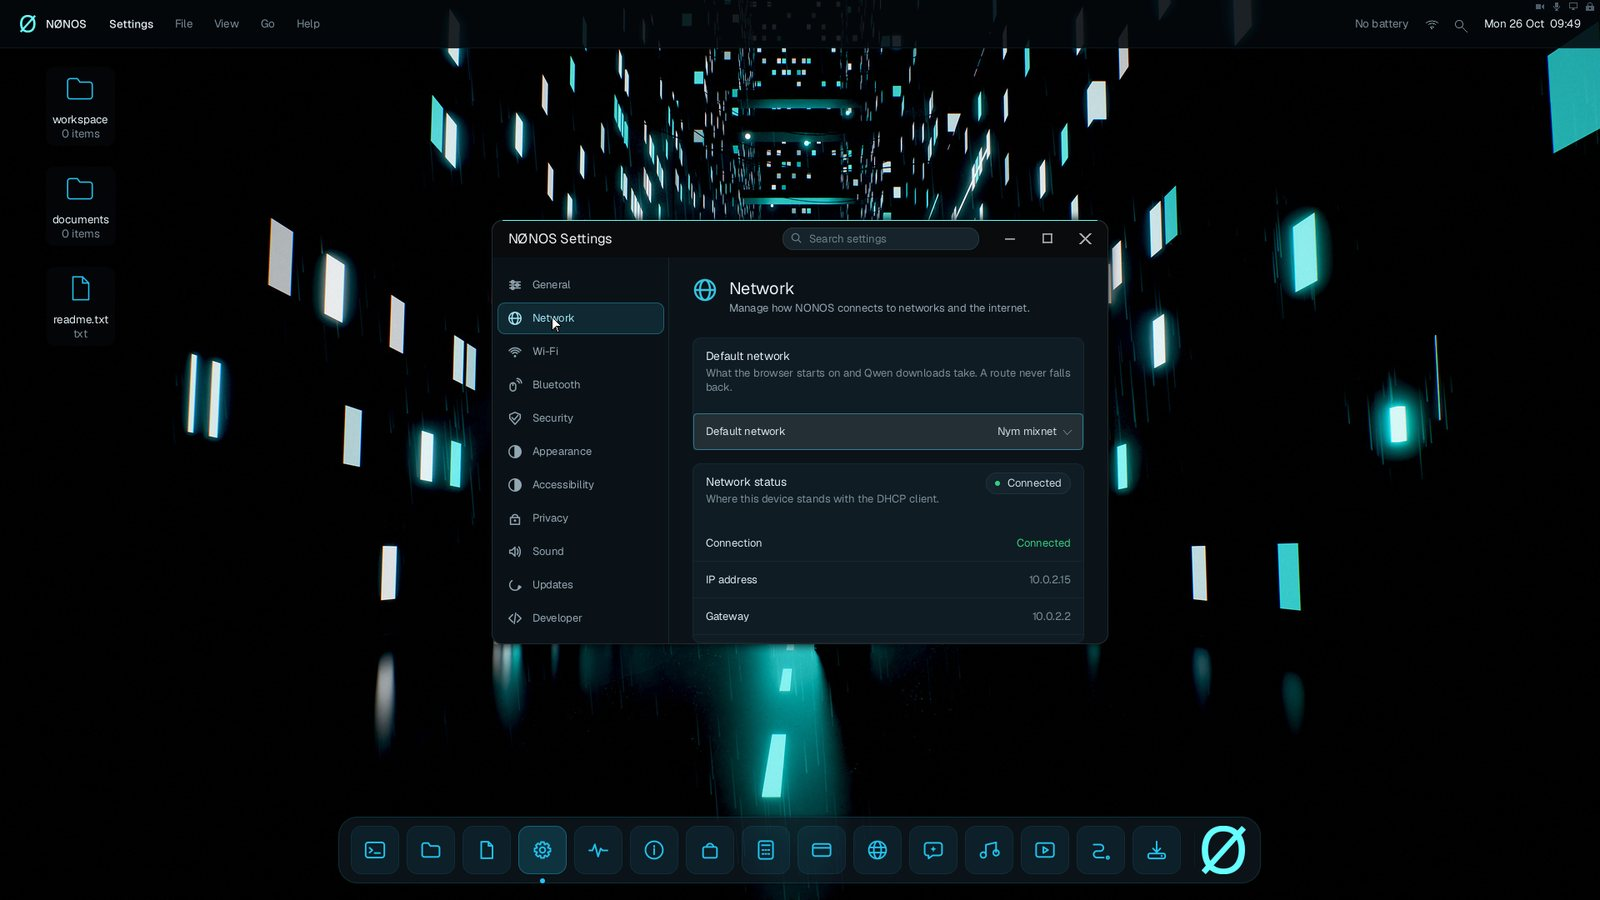
\includegraphics[width=\textwidth]{figures/settings-network.jpg}
\end{minipage}
\caption{Left, the first-boot step that picks the network the machine's traffic leaves through. Right, Settings, which shows the network in use and changes it. Both from the sealed 0.9.3 image under KVM, so Settings shows a virtual network, not a real one.}
\label{fig:routeshots}
\end{figure}

\subsection{What a Linux guest gets}

For a Linux program the route logic is the same code with one extra rule. A stream to anywhere outside the program's own family goes by the system's chosen network: Anyone to \code{net.anon}, Nym or an unreadable setting to the mixnet socket, and Direct also to the mixnet, because a guest is never given a direct socket. A chosen network that is not running is \code{ENETUNREACH}, and nothing else is tried.\src{userland/capsule_linux/src/linux/net/guest_route.rs:59-75} A program binds and listens only on 127.0.0.0/8; a datagram to outside the family is \code{ENETUNREACH}; a raw internet socket is \code{EPERM}.\src{userland/capsule_linux/src/linux/net/policy.rs:33-53}

\subsection{The transports}

Both transports are new \code{no\_std} code. \nonos{} links neither the Nym client nor a Tor or Anyone client.\src{docs/security/anonymity-transports.md} \code{net.nym} builds Sphinx \cite{sphinx} packets of 2,413 bytes for the Nym mixnet \cite{nym} with a 348-byte header across three mix layers and an exit gateway, and receives replies through single-use reply blocks. \code{net.anon} is a client for the Anyone network, a fork of Tor \cite{tor}: it checks consensus documents against directory-authority signatures, builds three-hop bandwidth-weighted circuits with the ntor handshake, and authenticates relays through Ed25519 certificates.\note{\path{docs/security/anonymity-transports.md}, section "Sphinx".} The browser, \code{curl}, \code{git} and the wallet use a \code{no\_std} TLS 1.3 client with the Mozilla root set.\src{docs/security/tls-and-certificates.md}

\subsection{What running traffic has shown}

0.9.2 had to say that no booted image had carried traffic through a live Nym gateway or Anyone circuit. 0.9.3 has some, and we say what and where.

On a KVM host, the Monero command-line wallet synced from the node named in its listing, \code{xmr-node.cakewallet.com:18081}, over Anyone and over Nym. In one Nym run the serial log counts 3,321 \code{[SOCKS5] exit answered} lines while the wallet synced; in another run a fresh wallet refreshed to 3,794,280 of 3,794,280 blocks and \code{exit} ended it with status 0. These were development images, and the install itself used the host's package relay, so the install shows nothing about the real mirror; the sync does show the route. The wallet's own window progress is quoted in the evidence from the notes of those runs, because a terminal run's output never reaches serial.\note{\path{docs/release-evidence/0.9.3/s1-g-kvm/README.md}; \path{docs/release/0.9.3-what-is-new.md}, section "The Monero wallet over Nym and Anyone".}

The same evidence is a good example of how these runs fail. An install over the real Alpine mirror stalled because the window opened three streams at once and both proxies keep one stream per caller, so each took the conversation from the one before and no package was answered. A lone stream carried the 24.7~MB Monero package whole. An install now fetches one package at a time. A failing first refresh on wallet open, "net.socks5 sent an answer this cannot read", is fixed on the host and has not been shown fixed on a boot, and the release notes tell the person to keep the seed on paper.\note{\path{docs/release-evidence/0.9.3/s1-g-kvm/README.md}; \path{docs/release/0.9.3-known-issues.md}, section "Linux apps".}

A separate capture on 25 October judged the egress of an idle first boot of a development image under QEMU. It holds 2,287 frames, 2,284 of them from the guest under one random locally administered MAC. Every peer the guest reached is pinned in the image: five Nym bootstrap gateways, Nym's directory API and seven Anyone directory authorities. There was no DNS, NTP, discovery packet or IPv6. That is the nearest thing to a test of the setup wizard's sentence, "Telemetry: NONOS has none, so there is no switch for it", and it comes with its own list of what it did not show: nobody opened an app, no relay appears in the capture, and real hardware and Wi-Fi are not covered.\note{\path{docs/security/privacy-guarantees.md}, section "Booted evidence"; \path{userland/capsule_setup_wizard/src/render/screens/privacy.rs:18}.}

\subsection{What the network design does not cover}

The kernel does not enforce the route in general. A capsule holding \code{Network} could call the TCP or socket services directly, and programs built on the toolchain's Rust \code{std} connect directly. Both transports start on every boot that starts networking, so the local network can see that a machine runs Nym and Anyone under every choice, including Direct.\src{docs/release/0.9.3-security-limits.md} Nym's directory is fetched over TLS from one validator without an operator signature, and cover traffic is sent only on request, which no program sets. \code{net.anon} has no vanguards, no conflux, no congestion control and no ntor v3, and does not check the digest in a relay's SENDME. Neither transport pads traffic on its own, and neither directory fetch is anonymous.\note{\path{docs/security/anonymity-transports.md}, section "What the transports lack".} The documentation page for the transports still says that no booted image has carried live traffic, which the evidence above contradicts; we follow the evidence and have noted the page for correction.\note{\path{docs/security/anonymity-transports.md}, section "What each transport reports".}

For Linux programs the position is better, because the route is enforced by the personality for guests and by the kernel for the instance that serves them (Section~\ref{sec:box}). For capsules in general it is a shared library and a convention that the capsules that hold \code{Network} follow.
